\chapter{Evaluación experimental}
\label{cap:evaluacionexperimental}
En el presente capítulo se presentan los resultados obtenidos de las diferentes implementaciones para los métodos propuestos en la secciones anteriores. Se comienza por la implementación de los métodos de procesamiento de transacciones de lectura, posteriormente se muestra los resultados obtenidos para los diferentes métodos de predicción de tiempos de respuestas para consultas y el comportamiento que tienen para diferentes conjuntos de datos. Finalmente se presenta el comportamiento de las estrategias de planificación presentadas para diferentes tipos de escenarios.

\section{Hardware y conjunto de datos}
\label{evaluacionexperimental:hardwareydatos}
Los experimentos fueron ejecutados en un Intel Xeon E5620 2.4 \textit{Ghz.} con 8 núcleos físicos, tecnología \textit{hyper-threading} y 90 gigabytes de memoria de acceso aleatorio (\textit{RAM}). Se utilizaron dos conjuntos de datos para llevar a cabo los experimentos, estos son frecuentemente usados por la comunidad del área de recuperación de información. El primero de ellos es \textit{GOV2}, este conjunto es una colección de aproximadamente 25 millones de páginas \textit{Web} obtenida desde los dominios \textit{.gov} y que pesa 426 \textit{GB}. La otra colección de datos utilizada es la \textit{ClueWeb09}, la cual fue creada para apoyar la investigación en recuperación de la información y las tecnologías relacioanadas con el lenguaje humano, consiste en alrededor de un billón de páginas en diez lenguajes diferentes y 50 millones en inglés. \textit{ClueWeb09} pesa alrededor de 5 \textit{TB} en forma comprimidad y 25 \textit{TB} descomprimida. 
% Las consultas (queries)

\section{Wand multithreaded}
\label{evaluacionexperimental:wm}
En esta sección se muestra la implementación de dos enfoques para el procesamiento de consultas a través del algoritmo Wand \citep{Broder:2003}. El primer enfoque es el esquema de \textit{heap} locales (LH), en el que cada hebra obtiene sus mejores documentos para una consulta dada y luego una hebra maestra se encarga de mezclar todos los resultados de cada uno de los hilos de ejecución para construir el conjunto \textit{top-K} final; el segundo enfoque es el enfoque de \textit{heap} compartido (SH), en el que se tiene un \textit{heap} visible a todos los hilos de ejecución y en donde ellos compiten por el acceso a esta estructura de datos. El detalle del diseño de los enfoques LH y SH están disponibles en \ref{scheduling:wlh} y \ref{scheduling:whc}. 

\subsection{Esquema LH}
\label{evaluacionexperimental:esquemalh}
En el esquema LH todos los hilos de ejecución tienen sus propias estructuras de datos y variables que soportan la resolución de una transacción de lectura. La clase \textit{TopKMultithreadWandOperatorLocal} es la encargada de administrar la lógica de ejecución, además prepara las variables e inicia los hilos de ejecución. El Código \ref{code:topkmultithreadwandoperatorlocal} muestra la implementación, en el que existe un método llamado \textit{execute}, este método es el encargado de llevar a cabo la resolución de la consulta, recibe como entrada la consulta a ser resuelta y un vector en el que se almacenará los resultados obtenidos. Adicionalmente, este método es el encargado de lanzar las hebras con que se resolverá cada consulta y a cada una de ellas le asigna un objeto de tipo \textit{TopKWandOperator} ($arr\_ops[pid\_thread]$) para obtener los resultados. Todo este proceso es llevado a cabo usando $K$ como tamaño del conjunto que se quiere obtener. Además se definen variables como \textit{$mapas\_ubs$}, el cual asocia a cada término los \textit{upper bounds} con los que el método Wand trabajará y \textit{$query\_partes$}, variable que define en cuántas partes la consulta debe ser dividida y está supeditada al número de hebras con que esta será resuelta.

\lstinputlisting[label=code:topkmultithreadwandoperatorlocal, caption=Implementación de la clase TopKMultithreadWandOperatorLocal.h, language=C++]{code/TopKMultithreadWandOperatorLocal.h}

En la Figura \ref{fig:esquema_ejecucion_wandlh} se ejemplifica la resolución de una consulta con cuatro hilos de ejecución. Una vez que el sistema asigna el número de hebras que se utilizará para la resolución de la consulta, esta es tomada por el objeto \textit{TopKMultithreadWandOperatorLocal} y hace un llamado al método \textit{execute}, en el que se hace una preparación de variables y se lanzan los hilos de ejecución; cada uno de ellos tiene asignado dos objetos: (1) \textit{TopKWandOperator}, el cual se encarga de que cada hilo de ejecución solo resuelva la parte de la consulta que se le asignó, y (2) \textit{Wand}, el cual se encarga de obtener los mejores $K$ documentos guardándolos en un \textit{heap}.

\begin{figure}[th!]
\centering
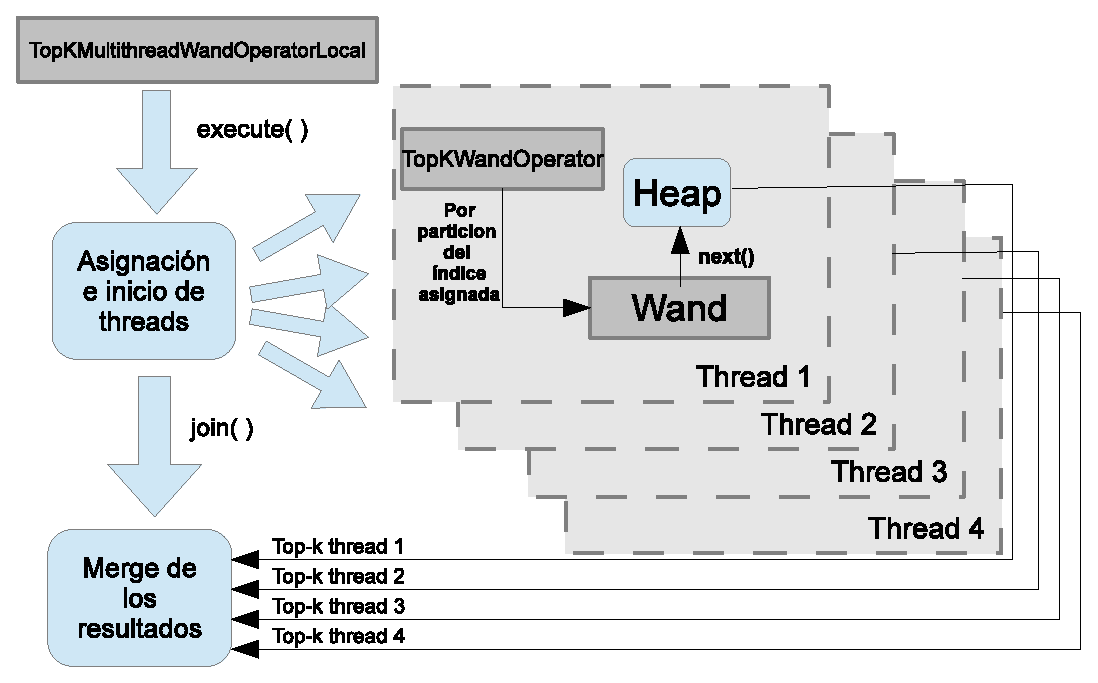
\includegraphics[scale=.75]{images/ejecucion_topkmultithreadwandopLOCAL.eps}
\caption{Esquema de ejecución enfoque LH.}
\label{fig:esquema_ejecucion_wandlh}
\end{figure}

\subsection{Esquema SH}
\label{evaluacionexperimental:esquemash}
En el esquema SH los hilos de ejecución trabajan con variables compartidas, incluído el \textit{heap} en donde se almacenan los resultados. La ejecución de este enfoque es llevada a cabo por la clase \textit{TopKMultithreadWandOperatorLocks}, lo cual se puede ver en el Código \ref{code:topkmultithreadwandoperatorlocks}; en esta implementación se puede observar la declaración de una clase anidada, la cual contiene las variables que serán compartidas por los hilos de ejecución. Dentro de las variables más importantes está el \textit{heap}, el umbral utilizado para decidir si un documento debe estar dentro del \textit{heap} y la variable de tipo \textit{mutex} que permite el acceso exclusivo a las variables compartidas. 

\lstinputlisting[label=code:topkmultithreadwandoperatorlocks, caption=Implementación de la clase TopKMultithreadWandOperatorLocks.h, language=C++]{code/TopKMultithreadWandOperatorLocks.h}

La Figura \ref{fig:esquema_ejecucion_wandsh} muestra un ejemplo de resolución de consulta utilizando cuatro hilos de ejecución y el enfoque SH. Al igual que en el esquema anterior, la clase principal inicializa variables e inicia los hilos de ejecución; el objeto \textit{TopKWandOperator} asignará a cada hebra la parte del índice invertido con la que cada hebra resolverá la consulta. Cada vez que un hilo de ejecución utilizando el objeto Wand encuentre un documento candidato para estar en el conjunto \textit{top-K} final, debe pedir acceso exclusivo a las estructuras de datos involucradas (\textit{heap} y umbral), de esta forma se evita resultados erróneos en el conjunto final producto del paralelismo entre los hilos de ejecución.  

\begin{figure}[th!]
\centering
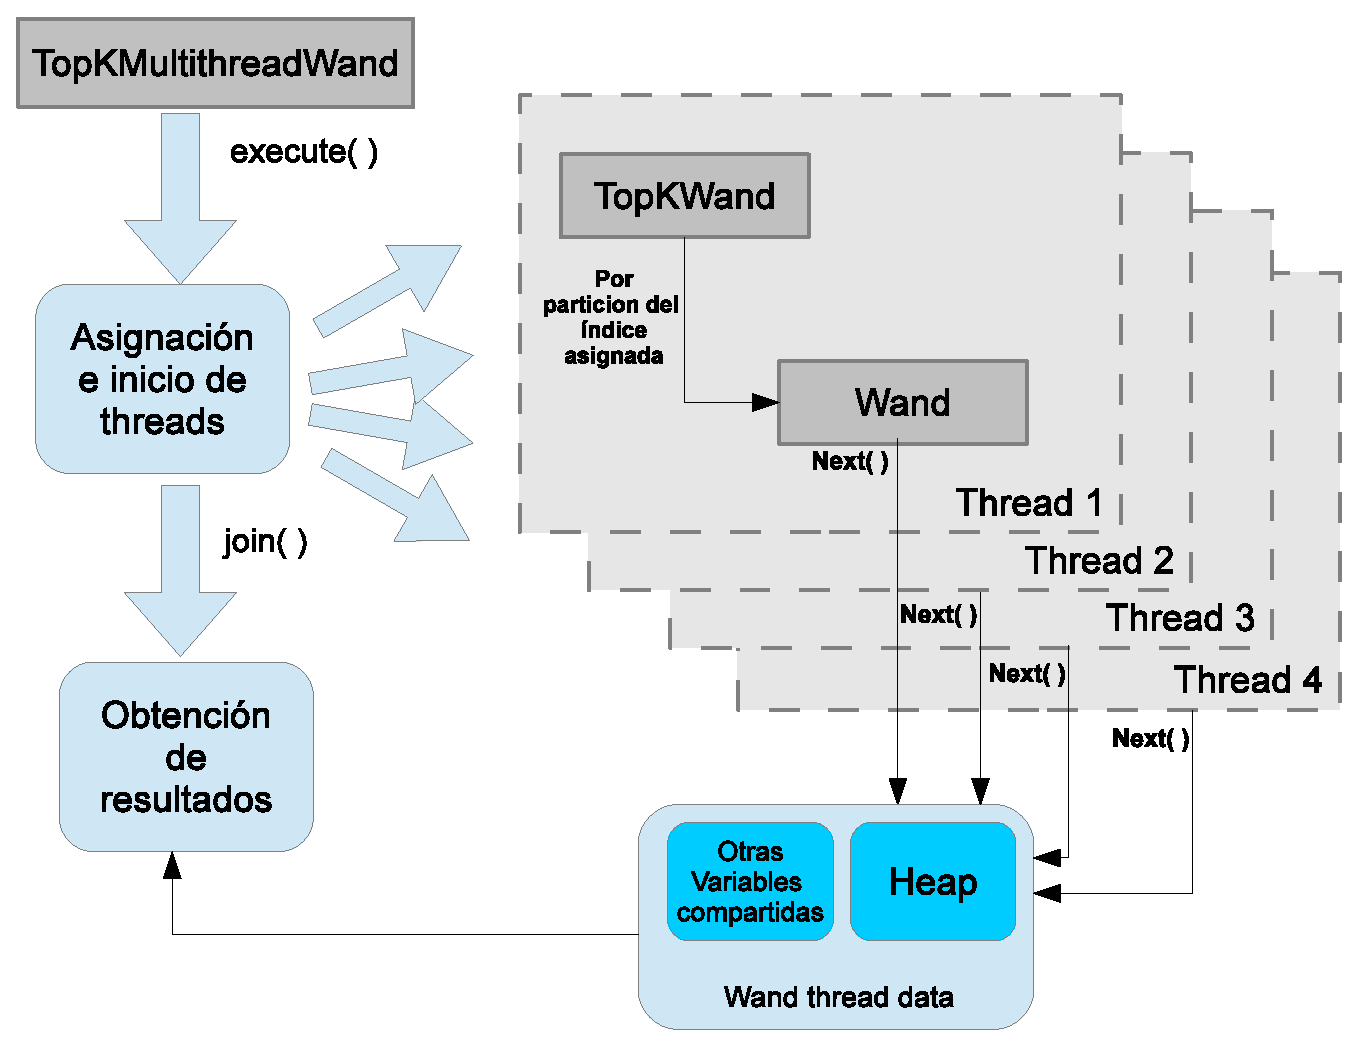
\includegraphics[scale=.75]{images/ejecucion_topkmultithreadwandopCOMPARTIDO.eps}
\caption{Esquema de ejecución enfoque SH.}
\label{fig:esquema_ejecucion_wandsh}
\end{figure}


\subsection{Resultados obtenidos}
\label{evaluacionexperimental:resultadosObtenidos}
En la Figura \ref{fig:tiempos_wand} se puede observar el tiempo promedio del enfoque LH y el enfoque SH en resolver un conjunto de 10,000 consultas de la colección \textit{GOV2}. A medida que crece el número de hilos de ejecución, el enfoque de \textit{heaps} compartidos toma ventaja por sobre el enfoque de \textit{heaps} locales, sin embargo, cuando se utiliza un hilo de ejecución se puede observar que LH ($117.486 ms$) requiere un tiempo menor que SH ($130.591 ms$), esto se debe porque en LH no se usan variables compartidas que retrasen a los hilos de ejecución esperando a que otros las liberen. LH requiere menos tiempo en resolver el \textit{log} de consultas para 2,4,8 y 16 hebras. 
El esquema LH puede estar muy supeditado a la distribución de documentos en las listas del índice invertido, ya que si un hilo de ejecución procesa su corrrespondiente parte del índice invertido en donde los mejores puntajes se encuentran al final, entonces el \textit{heap} tendrá un umbral bajo al comienzo del proceso, eso implica un proceso de descarte de documentos menos eficiente y el tiempo de ejecución requerido será mayor, retrasando el proceso que mezcla los resultados para obtener el conjunto \textit{top-K} final. 
Como el esquema SH ocupa un solo \textit{heap} para obtener los mejores $K$ documentos, el \textit{heap} tiende a llenarse rápidamente con los mejores documentos globales, esto implica que el puntaje mínimo del \textit{heap} (umbral) tiende a crecer rápidamente, permitiendo un mejor descarte de documentos y menor tiempo de ejecución para las hebras. 

\begin{figure}[!ht]
\centering
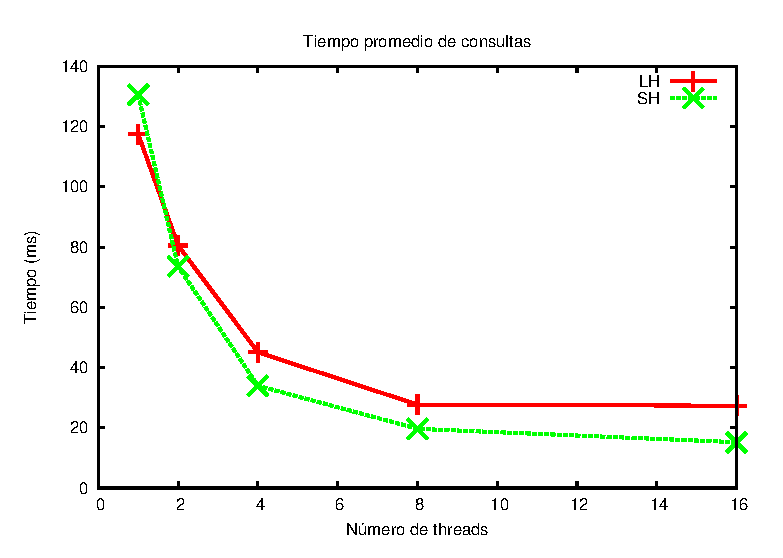
\includegraphics[scale=.75]{images/tiempos_wand.eps}
\caption{Tiempos promedios de las consultas.}
\label{fig:tiempos_wand}
\end{figure}

Adicionalmente en la Figura \ref{fig:eficiencias_wand} se puede ver en forma general que con la estrategia de enfoques compartidos se obtienen mejores eficiencias que con la estrategia LH. Con SH la mejor eficiencia que se obtiene es con 4 hilos de ejecución ($0.962$ ms), mientras que con 2 y con 8 hebras se obtiene una eficiencia de $0.887$ y $0.831$ milisegundos; en general se obtiene buenas eficiencias para 1,2,4 y 8 hebras, sin embargo, con 16 hilos de ejecución la eficiencia baja considerablemente ($0.5403$ ms) con respecto a las anteriores, esto se debe principalmente a la tecnología \textit{hyperthreading} de la máquina utilizada. También es interesante ver que el uso exclusivo del \textit{heap} compartido por parte de los \textit{threads} no tiene un fuerte impacto en el rendimiento. La eficiencia baja de LH se debe porque para obtener el conjunto \textit{top-K} final de una consulta debe haber una sincronización de todos los hilos de ejecución involucrados en que cada uno de ellos envíe sus \textit{top-K} locales a la hebra maestra, y además porque existe un costo adicional de calcular el conjunto \textit{top-K} final entre los $P \times K$ documentos seleccionados (siendo $P$ el número de procesadores). 
                     
%Para los siguientes experimentos del presente trabajo se ocupará el enfoque SH para resolver las transacciones de lectura.

\begin{figure}[!ht]
\centering
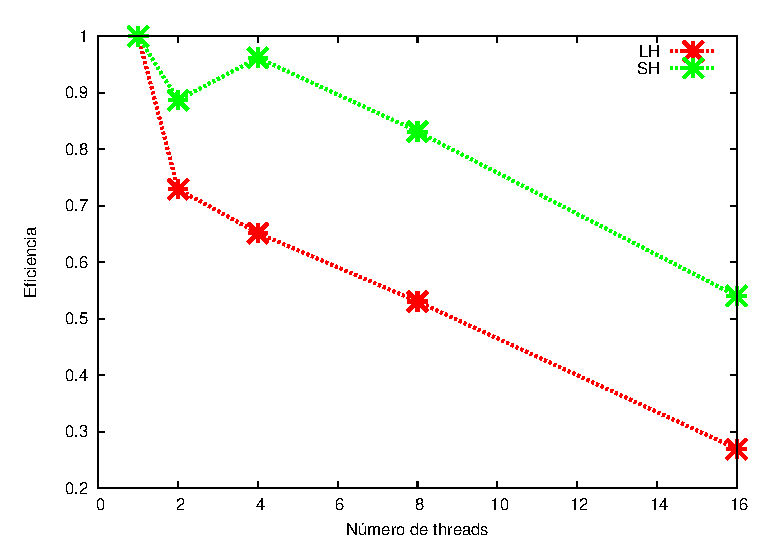
\includegraphics[scale=.75]{images/eficiencias_wand.eps}
\caption{Eficiencias para Wand con heaps compartido y locales.}
\label{fig:eficiencias_wand}
\end{figure}

\section{Predicción de tiempos}
\label{evaluacionexperimental:predicciontiempos}
% Demostrar que Regresión lineal es mejor

\section{Estrategias de scheduling}
\label{evaluacionexperimental:estrategiasscheduling}
Se compararon las estrategias de planificación por bloques \citep{Ye:2007} usando el predictor multilineal y además un predictor perfecto, el cual sabe de antemano el tiempo real de las consultas. Para determinar el número de hebras a ser usado para resolver cada consulta, el sistema predice el tiempo que esta tomará, y escoge el mínimo número de hebras necesarias con el que el tiempo predicho es menor o igual a la cota superior de tiempo establecida. Se experimentó con diferentes valores para fijar la cota superior y los mejores resultados fueron obtenidos con el tiempo promedio de las consultas. Se puede observar en la Figura X que un mejor predictor puede conducir a mejores tiempos de ejecución. Adicionalmente se analiza el comportamiendo que tienen estas estrategias al responder consultas divididas en conjuntos de diferentes tamaños (1000, 500, 200, 100 and 50). En cada caso las técnicas procesaron todas las consultas con una pausa entre lotes, el tiempo de ejecución total tomado corresponde a la suma de tiempos de ejecución de los lotes. El mejor resultado fue obtenido por la estrategia Times Ranges usando el predictor perfecto. 
% Hacer un análisis del tiempo y el tamaño de los bloques

%%% FIGURA 6 PAPER PDP

En base a experimentación se ha encontrado que en general procesar transacciones de lectura utilizando Wand bajo un enfoque de bloques \citep{Ye:2007} es menos eficiente con respecto a otros enfoques. Es por esta razón que en las siguientes experimentaciones y comparaciones solo se utiliza la estrategia \textit{Times Ranges} con predictor perfecto.

% Se dejan afuera todas las otras estrategias de planificación por bloques, exepto Times Ranges.

% Se Compara el mejor de bloques: Times Ranges con estrategia de 1TQ y QueryUnits

Para observar el comportamiento de la estrategia 1TQ se utiliza una versión de la estrategia unidades de trabajo haciendo uso de una sola unidad de procesamiento por cada consulta, de esta manera las hebras trabajan de forma independiente sobre diferentes transacciones de lectura y es equivalente a la estrategia 1TQ mostrada en la sección \ref{scheduling:baseline}. Adicionalmente se observa el comportamiento que tiene el enfoque de unidades de trabajo en diferentes versiones (1) Se asigna a las consultas que llegan al sistema un número fijo de unidades de trabajo, y (2) Utilizando el predictor multilineal perfecto para predecir el número de unidades de trabajo. 

Los resultados obtenidos se pueden ver en la Figura Y, en donde...


% Mostrados que Times Ranges es mejor que todos los demás bloques y que TimesRanges es malo


% Comparación de diferentes técnicas con respecto al número de threads disponibles para el caso de batches de 50 queries








